\documentclass[english,11pt, reqno, oneside]{amsart}
\usepackage{amsmath}
\usepackage{amssymb}
\usepackage[usenames,dvipsnames]{xcolor}
\usepackage[colorlinks=true,linkcolor=blue!95!black, citecolor = green!55!black,bookmarksdepth=3]{hyperref}
\usepackage{tikz}
\usetikzlibrary{calc}
\usetikzlibrary{math}
\usetikzlibrary{decorations.markings, decorations.pathreplacing,shapes.misc}

\begin{document}

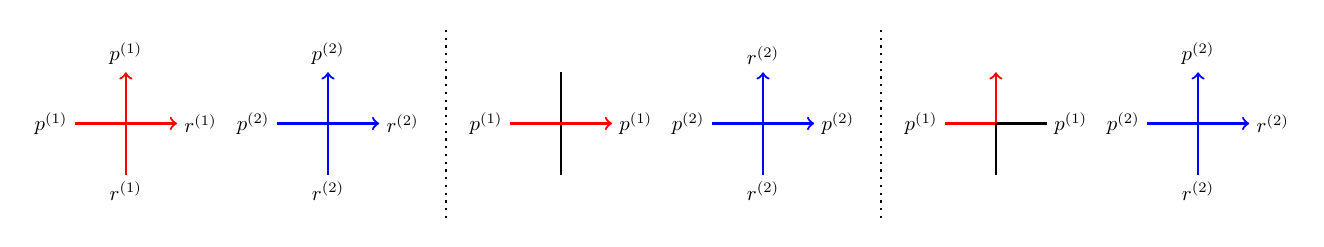
\begin{tikzpicture}[scale=0.65]
  \draw[red, thick] (-1,0) -- ++(1,0);
  \draw[red, thick, ->] (0,0) -- ++(1,0);
  \draw[red, thick] (0,-1) -- ++(0,1);
  \draw[red, thick, ->] (0,0) -- ++(0,1);

  \node[anchor=east, scale=0.75] at (-1,0) {$p^{(1)}$};
  \node[anchor=north, scale=0.75] at (0,-1) {$r^{(1)}$};

  \node[anchor=west, scale=0.75] at (1,0) {$r^{(1)}$};
  \node[anchor=south, scale=0.75] at (0,1) {$p^{(1)}$};  

  \begin{scope}[shift={(3.95,0)}]
  \draw[blue, thick] (-1,0) -- ++(1,0);
  \draw[blue, thick, ->] (0,0) -- ++(1,0);
  \draw[blue, thick] (0,-1) -- ++(0,1);
  \draw[blue, thick, ->] (0,0) -- ++(0,1);

  \node[anchor=east, scale=0.75] at (-1,0) {$p^{(2)}$};
  \node[anchor=north, scale=0.75] at (0,-1) {$r^{(2)}$};

  \node[anchor=west, scale=0.75] at (1,0) {$r^{(2)}$};
  \node[anchor=south, scale=0.75] at (0,1) {$p^{(2)}$};  
  \end{scope}

  \draw[dotted, thick] (6.25,-1.85) -- ++(0,3.7);


\begin{scope}[shift={(8.5,0)}]
  \draw[thick] (0,-1) -- ++(0,1);
  \draw[thick] (0,0) -- ++(0,1);
  \draw[red, thick] (-1,0) -- ++(1,0);
  \draw[red, thick, ->] (0,0) -- ++(1,0);

  \node[anchor=east, scale=0.75] at (-1,0) {$p^{(1)}$};

  \node[anchor=west, scale=0.75] at (1,0) {$p^{(1)}$};

  \begin{scope}[shift={(3.95,0)}]
  \draw[blue, thick] (-1,0) -- ++(1,0);
  \draw[blue, thick, ->] (0,0) -- ++(1,0);
  \draw[blue, thick] (0,-1) -- ++(0,1);
  \draw[blue, thick, ->] (0,0) -- ++(0,1);


  \node[anchor=east, scale=0.75] at (-1,0) {$p^{(2)}$};
  \node[anchor=north, scale=0.75] at (0,-1) {$r^{(2)}$};

  \node[anchor=west, scale=0.75] at (1,0) {$p^{(2)}$};
  \node[anchor=south, scale=0.75] at (0,1) {$r^{(2)}$};  
  \end{scope}

  \draw[dotted, thick] (6.25,-1.85) -- ++(0,3.7);
\end{scope}


\begin{scope}[shift={(17,0)}]
  \draw[red, thick] (-1,0) -- ++(1,0);
  \draw[thick] (0,0) -- ++(1,0);
  \draw[thick] (0,-1) -- ++(0,1);
  \draw[red, thick, ->] (0,0) -- ++(0,1);


  \node[anchor=east, scale=0.75] at (-1,0) {$p^{(1)}$};

  \node[anchor=west, scale=0.75] at (1,0) {$p^{(1)}$};

  \begin{scope}[shift={(3.95,0)}]
  \draw[blue, thick] (-1,0) -- ++(1,0);
  \draw[blue, thick, ->] (0,0) -- ++(1,0);
  \draw[blue, thick] (0,-1) -- ++(0,1);
  \draw[blue, thick, ->] (0,0) -- ++(0,1);


  \node[anchor=east, scale=0.75] at (-1,0) {$p^{(2)}$};
  \node[anchor=north, scale=0.75] at (0,-1) {$r^{(2)}$};

  \node[anchor=west, scale=0.75] at (1,0) {$r^{(2)}$};
  \node[anchor=south, scale=0.75] at (0,1) {$p^{(2)}$};  
  \end{scope}
\end{scope}
\end{tikzpicture}

\end{document}